\documentclass[11pt,xcolor=x11names,compress]{beamer}

%\usetheme{Berlin}
\usepackage{cmap}					% поиск в PDF
\usepackage{mathtext} 				% русские буквы в формулах
\usepackage[T2A]{fontenc}			% кодировка
\usepackage[utf8]{inputenc}			% кодировка исходного текста
%\usepackage[english,russian]{babel}	% локализация и переносы
\usepackage{array}
\usepackage{amsmath,amsfonts,amssymb,amsthm,mathtools} % AMS

%%% Работа с картинками
\usepackage{graphicx}  % Для вставки рисунков
%\usepackage{booktabs}% Для вставки таблиц
%%% Картинки
\usepackage{tikz} % Работа с графикой
\usetikzlibrary{decorations.fractals}
\usepackage{pgfplots}
\usepackage{pgfplotstable}
\usepackage[textfont={footnotesize}]{caption}

%% Beamer Layout %%%%%%%%%%%%%%%%%%%%%%%%%%%%%%%%%%
\useoutertheme[subsection=false,shadow]{miniframes}
\useinnertheme{default}
\usefonttheme{serif}
\usepackage{palatino}
\usepackage{color}
\usepackage{amsmath}


\setbeamerfont{title like}{shape=\scshape}
\setbeamerfont{frametitle}{shape=\scshape}

\setbeamercolor*{lower separation line head}{bg=green} 
\setbeamercolor*{normal text}{fg=black,bg=white} 
\setbeamercolor*{alerted text}{fg=red} 
\setbeamercolor*{example text}{fg=black} 
\setbeamercolor*{structure}{fg=black} 
 
\setbeamercolor*{palette tertiary}{fg=black,bg=black!10} 
\setbeamercolor*{palette quaternary}{fg=black,bg=black!10} 

\setbeamertemplate{footline}[frame number]
\setbeamerfont{page number in head/foot}{size=\normalsize}
\setbeamertemplate{caption}{\raggedright\insertcaption\par}

\DeclareMathOperator*{\argmin}{arg\,min}
\DeclareMathOperator{\E}{\mathbb{E}}

\renewcommand{\(}{\begin{columns}}
\renewcommand{\)}{\end{columns}}
\newcommand{\<}[1]{\begin{column}{#1}}
\renewcommand{\>}{\end{column}}
%%%%%%%%%%%%%%%%%%%%%%%%%%%%%%%%%%%%%%%%%%%%%%%%%%




\captionsetup{justification=centering}
\setbeamertemplate{bibliography item}[text]
\bibliographystyle{apalike}

%\captionsetup{font=scriptsize,labelfont=scriptsize}

\title{\textbf{Vector representation of large DNA and protein strings}}
\date{
	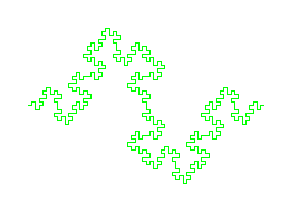
\begin{tikzpicture}[decoration=Koch curve type 2] 
		\draw[green] decorate{ decorate{ decorate{ (0,0) -- (3,0) }}}; 
	\end{tikzpicture}  
	\\
	\vspace{1cm}
	\today
}
\author{Bogdan Kirillov \and Phan Duc \and Evgenij Baraboshkin}
\institute{Skolkovo Institute of Science and Technology}
\usepackage{graphicx}
\begin{document}
\maketitle

\begin{frame}
	\frametitle{The key papers to use}
	\begin{itemize}
		\item Dna2vec: Consistent vector representation of variable-length k-mers, Ng,P -- the one we are to discuss here;
		\item Distributed Representations for Biological Sequence Analysis, Kimothi et al., ;
		\item Continuous Distributed Representation of Biological Sequences for Deep Genomics and Deep Proteomics, Asgari, E. and Mofrad, M;
	\end{itemize}
\end{frame}

\begin{frame}
	\frametitle{Bioinformatics 101}
	\scriptsize
	Biological data are complex!
	\begin{itemize}
		\item Direct Data Augmentation is not really applicable;
		\item Working with really large (1Mb and more) DNA sequences is unclear;
		\item Unlike basic CV, there usually are no clue about how well we can solve the problem with given training/testing data;
		\item A lot of experiments are low-throughput so sample sizes can be limited and the samples may overlap;
	\end{itemize}
	\begin{columns}
	\begin{column}{0.5\textwidth}
		\begin{figure}
			\caption*{\tiny{Augmentation in Computer Vision}}
			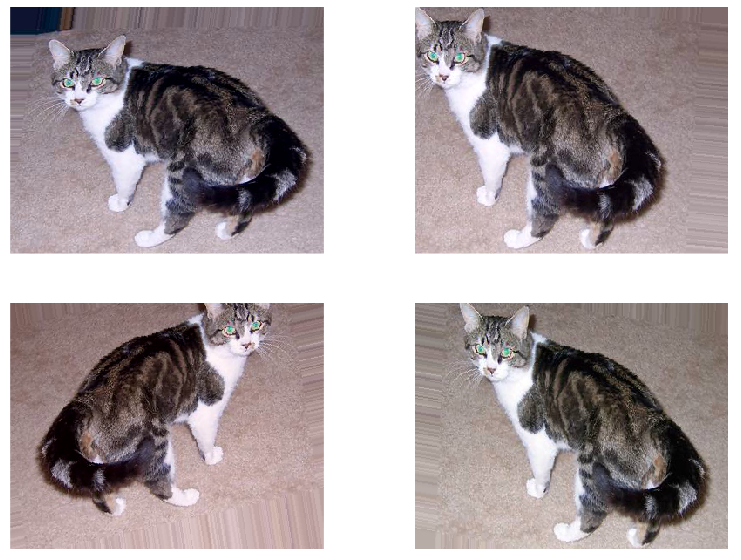
\includegraphics[width=0.65\textwidth]{statement1.png}
			\caption*{\tiny{Cropped and mirrored cat pic remains a cat pic}}
		\end{figure}
	\end{column}
	\begin{column}{0.5\textwidth}
		\begin{figure}
			\caption*{\tiny{Biological sequence case}}
			
\includegraphics[width=0.65\textwidth]{statement2.png}
			\caption*{\tiny{You can't say the same here}}
		\end{figure}
	\end{column}
	\end{columns}
\end{frame}

\begin{frame}
	\frametitle{Word embeddings and their use for DNA/Proteins}
	\begin{figure}
		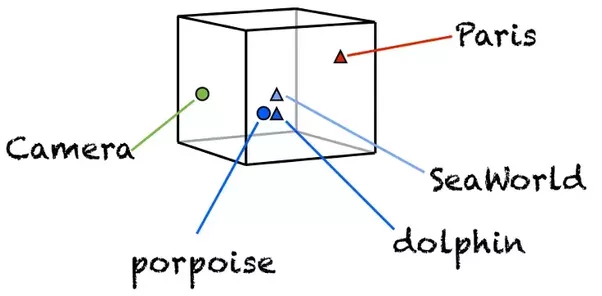
\includegraphics[width=\textwidth]{word_embeddings.png}
		\caption*{\tiny{Example of word embedding}}
	\end{figure}
\end{frame}


\begin{frame}
	\frametitle{Problem of k-mer length choice}
\end{frame}

\begin{frame}
	\frametitle{dna2vec training procedure}
\end{frame}

\begin{frame}
	\frametitle{Stage 1: Long non-overlapping DNA fragments}
\end{frame}

\begin{frame}
	\frametitle{Stage 2: Overlapping variable-length k-mers}
\end{frame}

\begin{frame}
	\frametitle{Stage 3: Two-layer neural network}
\end{frame}

\begin{frame}
	\frametitle{Stage 4: Decompose aggregated model by k-mer lengths}
\end{frame}

\begin{frame}
	\frametitle{Alignment similarity}
\end{frame}

\begin{frame}
	\frametitle{Possible applications}
\end{frame}

\begin{frame}
	\frametitle{What can be improved?}
\end{frame}


\end{document}